%!TeX spellcheck = en_GB
% Die erste (unkommentierte) Zeile im Dokument legt immer die
% Dokumentklasse fest
\documentclass{scrartcl} 

% Präambel:
% Einbinen von zusätzlichen Paketen. Falls für eine Datei keine Endung
% explizit angegeben wird, benutzt LaTeX '.tex'. Im Folgenden wird
% also die Datei 'edv_pakete.tex' eingebunden.
% Die erste Zeile im Dokument legt immer die Dokumentklasse fest
%\documentclass[notitlepage]{scrreprt}
    % Die wichtigsten Dokumentklassen:
    %   scrbook, scrreprt, scrartcl, beamer, standalone
    % Einige gängige Optionen für \documentclass:
    %   ngerman
    %   titlepage, notitlepage
    %   onecolumn, twocolumn
    %   oneside, twoside
    %wird in Hauptdatei festgelegt

% Präambel

% Einige KOMA-Script-Optionen
\KOMAoptions{fontsize=12pt,paper=a4}      %Schriftgröße, Papierformat
\KOMAoptions{DIV=11}                      % Parameter mit dem man den Seitenrand ändern kann
\KOMAoptions{listof=totoc}

% Hier werden einige Pakete eingebunden
\usepackage[utf8]{inputenc}               % Direkte Eingabe von ä usw. Input=Eingabe
\usepackage[T1]{fontenc}                  % Font Kodierung für die Ausgabe Font=Ausgabe
\usepackage[english]{babel}               % Verschiedenste sprach-spezifische Extras, ngerman für neue deutsche Rechtschreibung, auch UK oder US möglich
\usepackage[autostyle=true]{csquotes}     % Intelligente Anführungszeichen, arbeitet mit Babel zusammen
%

\usepackage{amsmath}%Mathedarstellung
\usepackage{commath}%Mathedarstellung
\usepackage{physics}%Physik-Symbole
%\usepackage{IEEEtrantools}%IEEEeqnarray
%
\usepackage{siunitx}   % Intelligentes Setzen von Zahlen und Einheiten
%\sisetup{locale = DE}  % Deutsch als locale für die Zahlen und Einheiten
%http://tex.stackexchange.com/questions/2291/how-do-i-change-the-enumerate-list-format-to-use-letters-instead-of-the-defaul

\usepackage{enumitem}%erlaubt u.A. die Aufzählung mit Buchstaben, gefunden auf http://tex.stackexchange.com/questions/2291/how-do-i-change-the-enumerate-list-format-to-use-letters-instead-of-the-defaul
%
\usepackage[varg]{txfonts}                % Schönere Schriftart, muss nach amsmath, damit keine Fehlermeldung kommt
\usepackage{graphicx} %einbinden von Figuren/Bildern
\graphicspath{{figs/}} % Stammverzeichnis der verwendeten Bilder, muss im selben Ordner wie Hauptdatei sein
%
\usepackage[backend=biber, style=numeric, sorting=none]{biblatex}
%Verwenden von \cite in \footnote: Bibliographie drucken lassen, mehrmals kompilieren
\usepackage{hyperref}%erzeugt klickbare Elemente
\usepackage[all]{hypcap}%hyperref-befehle springen zum oberen Rand des Bildes
% Zum Einbinden von Programmcode verwenden wir das listings-Paket
\usepackage{listings}

% Für Syntax-Highlighting:
\usepackage{xcolor}

\usepackage{longtable}

% Die folgenden listings-Einstellungen sind nötig, um
% deutsche Umlaute und die Tilde (~) in listings-Umgebungen
% verwenden zu können.
\lstset{
    basicstyle=\ttfamily,    
    literate={~} {$\sim$}{1} % set tilde as a literal
    {ö}{{\"o}}1
    {ä}{{\"a}}1
    {ü}{{\"u}}1
    {ß}{{\ss}}1
    {Ö}{{\"O}}1
    {Ä}{{\"A}}1
    {Ü}{{\"U}}1
}

% Farben für Code-Syntaxhighlighting und Weiteres festlegen:
\lstset{
    % Keine besondere Markierung für Leerzeichen in Codes
    showspaces=false,               
    showstringspaces=false,         
    % Farebn für Code-Kommentare und Schlüsselworte:
    commentstyle=\color{red},       % comment style
    keywordstyle=\color{blue},      % keyword style
    stringstyle=\color{orange},		% string style
    breaklines=true,
    numbers=left,                    % where to put the line-numbers; possible values are (none, left, right)
    numbersep=5pt,                   % how far the line-numbers are from the code
    stepnumber=5, 					%how often there are line numbers in code listings
    tabsize=4, 						%default tabsize set to 4 spaces
    %language=python,
    }
%gefunden auf https://en.wikibooks.org/wiki/LaTeX/Source_Code_Listings
%eigene Kommandos/Abürzungen
\newcommand{\tb}{\textbackslash}
\newcommand{\txt}{\texttt}
\newcommand{\umt}{u_{(i+i\%2)/2}^{(2a)}}
\newcommand{\utmt}{u_{(i-2+i\%2)/2}^{(2a)}}
\newcommand{\uti}{\tilde{u}_i^{(a)}}
\newcommand{\utio}{\tilde{u}_{i-1}^{(a)}}




% Verzeichnisse mit Abbildungen; kann gestrichen werden,
% falls Sie dies schon in edv_pakete.tex definiert haben:
%\graphicspath{{../report}}

\addbibresource{refs.bib} %Hinzufügen einer Literaturdatenbank aus dem angegebenen Verzeichnis

% Titel, Autor und Datum
\title{Computational Physics}
\subtitle{Exercise 3}
\date{\today}
\author{Christiane Groß, Nico Dichter}

% Jetzt startet das eigentliche Dokument
\begin{document}
	\maketitle
\section{The long range Ising model}
We want to look at the long range Ising model, where an interaction with all other lattice points is considered. The theory was given in the lectures and on the exercise sheet. Inserting $\hat{J}=J/N$ to get normalizable solutions, we have: 
\begin{equation}
H_I(s)=-\frac{1}{2}\hat{J}\sum_{i,j}s_is_j-h\sum_{i,j}s_i
\label{eq:hamiltonianising}
\end{equation}

To be able to use HMC, we need to work in continuous space and the derivations on the sheet give us for $J>0$, using the Hubbard-Stratonovich-transformation:

\begin{equation}
Z=\sum_{\{s_i=\pm1\}}\exp(-\beta H_I(s,h))=
\int_{-\infty}^{\infty}\frac{\mathrm{d} \phi}{\sqrt{2\pi\beta\hat{J}}}
\exp\left( -\frac{\phi^2}{2\beta\hat{J}}+N\log\left( 2\cosh(\beta h\pm\phi)\right) \right) 
\label{eq:partfunc}
\end{equation}


We always choose $+\phi$ in the argument of the $\cosh$ and introduce the artificial action:
\begin{equation}
S(\phi)=\frac{\phi^2}{2\beta\hat{J}}-N\log\left( 2\cosh(\beta h+\phi)\right)
\end{equation}

and the artificial Hamiltonian:
\begin{equation}
H(\phi, p)=\frac{p^2}{2}+S(\phi)
\end{equation}

In this system, we can calculate Observables through: 
\begin{equation}
\langle O\rangle=\frac{1}{Z}\int_{-\infty}^{\infty}\frac{\mathrm{d} \phi}{\sqrt{2\pi\beta\hat{J}}}O(\phi)\exp(-S(\phi))
\label{eq:observable}
\end{equation}

\section{Deliberations}

\subsection{Observables}
We need to transform our observables into continuous functions of $\phi$.

\[\begin{array}{>{\displaystyle}r>{\displaystyle}c>{\displaystyle}l}

Z&=&\int_{-\infty}^{\infty}\frac{\mathrm{d} \phi}{\sqrt{2\pi\beta\hat{J}}}exp(-S(\phi))\\

%\langle O\rangle&=&\frac{1}{Z}\int_{-\infty}^{\infty}\frac{\mathrm{d} \phi}{\sqrt{2\pi\beta\hat{J}}}O(\phi)\exp(-S(\phi))\\

\dpd{\log(Z)}{x}&=&\frac{1}{Z}\dpd{Z}{x}=
-\frac{1}{Z}\int_{-\infty}^{\infty}\frac{\mathrm{d} \phi}{\sqrt{2\pi\beta\hat{J}}}\exp(-S(\phi))%\dpd{S(\phi)}{x}\\
\left( \dpd{S(\phi)}{x}-\sqrt{2\pi\beta\hat{J}}\dpd{}{x}\frac{1}{\sqrt{2\pi\beta\hat{J}}}\right) \\

\langle m\rangle&=&\frac{1}{Z}\int_{-\infty}^{\infty}\frac{\mathrm{d} \phi}{\sqrt{2\pi\beta\hat{J}}}m(\phi)\exp(-S(\phi))\\
&=&\frac{1}{N\beta}\dpd{\log(Z)}{h}=
-\frac{1}{NZ\beta}\int_{-\infty}^{\infty}\frac{\mathrm{d} \phi}{\sqrt{2\pi\beta\hat{J}}}\dpd{S(\phi)}{h}\exp(-S(\phi))\\

\Rightarrow m(\phi)&=&-\frac{1}{N\beta}\dpd{S(\phi)}{h}\\
&=&(-)^2\frac{1}{N\beta}\frac{2N\beta\sinh(\beta h+\phi)}{2\cosh(\beta h+\phi)}\\
&=&\tanh(\beta h+\phi)\\


\end{array}\]
\[\begin{array}{>{\displaystyle}r>{\displaystyle}c>{\displaystyle}l}

\text{analoguously } \langle \epsilon\rangle&=&-\frac{1}{N}\dpd{\log(Z)}{\beta}=
(-)^2\frac{1}{NZ}\int_{-\infty}^{\infty}\frac{\mathrm{d} \phi}{\sqrt{2\pi\beta\hat{J}}}\exp(-S(\phi))%\dpd{S(\phi)}{\beta}\\
\left( \dpd{S(\phi)}{\beta}-\sqrt{2\pi\beta\hat{J}}\dpd{}{\beta}\frac{1}{\sqrt{2\pi\beta\hat{J}}}\right)\\

\Rightarrow \epsilon(\phi)&=&\frac{1}{N}\left( \dpd{S(\phi)}{\beta}-\sqrt{2\pi\beta\hat{J}}\dpd{}{\beta}\frac{1}{\sqrt{2\pi\beta\hat{J}}}\right)\\
%\Rightarrow \epsilon(\phi)&=&\frac{1}{N} \dpd{S(\phi)}{\beta}\\
&=&-\frac{\phi^2}{2\beta^2 N\hat{J}}-\frac{2Nh\sinh(\beta h+\phi)}{N2\cosh(\beta h+\phi)}+\frac{2\pi\hat{J}}{2N\cdot2\pi\hat{J}\beta}\\

&=&-h\tanh(\beta h+\phi)-\frac{\phi^2}{2\beta^2 N\hat{J}}+\frac{1}{2N\beta}\\

\Rightarrow \beta\epsilon(\phi)&=&-\beta h\tanh(\beta h+\phi)-\frac{\phi^2}{2\beta N\hat{J}}+\frac{1}{2N}\\

\end{array}\]

We can insert these definitions into our code. We will not calculate $\langle \epsilon\rangle$ but instead $\langle \beta\epsilon\rangle$, because this allows us to absorb $\beta$ into $\hat{J}$ and $h$, and is also the form of the analytical solutions given on the sheet.



\subsection{Equations of Motion}

To be able to use HMC, we need to evolve $p$ and $\phi$ along a trajectory along which $H$ is approximately constant. We do this by integrating over the equations of motion:

\[\begin{array}{>{\displaystyle}r>{\displaystyle}c>{\displaystyle}l}
\dot{p}&=&-\dpd{H}{\phi}\\
&=&\frac{\phi}{\beta \hat{J}}-N\tanh(\beta h+\phi)\\
\dot{\phi}&=&\dpd{H}{p}=p
\end{array}\]

\subsection{HMC}

We want to calculate integrals like in eq.~\ref{eq:observable}. To do this, we want to generate  a Markov-Chain that has the stationary distribution $\exp(-S(\phi))/\sqrt{2\pi\beta\hat{J}}$, which we do with the Hybrid Monte Carlo algorithm as described on the sheet. First, we choose a $p$ randomly sampled from a normal distribution, calculate the artificial Hamiltonian $H(p, \phi)$ and evolve $p, \phi$ with the equations of motion with the help of a molecular dynamic integrator. We propose this change in $p,\phi$ and calculate the new Hamiltonian. We then accept this proposal with the Probability $\min(1, \exp(-\Delta H))$. As shown in the lectures this ensures our $\phi$ follow the desired distribution after a thermalisation phase.

\subsection{Leapfrog}

When evolving the equations of motion, we use the leapfrog integrator, as described on the sheet: One step in the integral means taking the variable $x$ to $x'=x+\epsilon\dpd{x}{t}$. We want to evolve both $p$ and $\phi$ and do this by using results from the step of one variable to evolve the other. We start with a half-step in $\phi$, then do $N_{md}-1$ combinations of one step in $p$ and one step in $\phi$ and end with a last step in $p$ and a last half-step in $\phi$, so we have done $N_{md}$ steps in both variables.

\subsection{Error estimation}
When determining errors for our measurements, we use binning and bootstrapping instead of the naive standard deviation. 
We do this as described in the lecture: First, we bin our data $O_i$ from $N$ measurements in $\lfloor N/l\rfloor$ bins $O^B_i=\frac{1}{l}\sum_{k=1}^l O_{(i-1)\cdot l+k}$. 

From these new datapoints, we make $R$ bootstrap replicas. For each replica, we sample with replacement from the given $O_i^B$, and take the arithmetic mean over those chosen values to be the replica. At the end, we can estimate the mean and error of our measurements as the arithmetic mean and standard deviation over $R$ bootstrap replicas.

This ensures we minimize the effects of correlation on our data and also get a realisitic error estimate.
%Binning to reduce correlation
%Bootstrap to estimate error

\section{Simulation}
Our code is in the github-repo \url{https://github.com/christianegross/CompPhys\_2021}. The simulation itself is in Exercise3/src/main/main.c, the gnuplotscript, wehere we have also implemented the expectations for the magnetization and energy are in Exercise3/report/plot.gp.

In the implementation of the simulation gsl\_vector objects  and views on these are used to accomplish proper binning (see \cite{gsldoc_mat}). 

At first the convergence of the leap frog algorithm is tested and the result is shown in fig. \ref{fig:converge}. Then for each parameter set (N,J) ($h=0.5$ fixed) a large amount of thermalization steps are made and afterwards several measurements of the wanted physical variable take place. A step in this case means to sample a conjugated momentum from the normal distribution and performing the leap frog algorithm with this momentum. Afterwards the relative change in total energy is calculated and an accept/reject takes place with the acceptance probability of:
\begin{equation}
	P_{acc.}=\min(1,\exp(\cal{H} (\texttt{q},\phi)-\cal H (\texttt{q}',\phi')))
\end{equation} 
It has to be noted, that in case of rejection the configuration $\phi$ gets added again to the list of generated configurations.
The thermalization steps are needed to make sure the measurements take place on configurations which resemble the given parameter set. The generation of the initial set of observables take place after each step. To lower the correlation binning was used on top of this initial set. At the end bootstrap was used to estimate an appropriate error on top of the binned data.

\subsection{Choosing bin length}

We do some pre-measurements with many bin lenghts and compare the resulting errors, plotted in fig.~\ref{fig:bootstrap}.

We see that for most $J$ the errors do not vary much with the bin length, they only rise a bit. For $J=0.4$ we see a big change in the error, but it plateaus staring at bn length 32. To ensure we are in this plateauing region, we choose the bin length $64$ for all our future analysis.

%The errors are quite small for all $N$, but for smaller $N$, but they rise for smaller $N$.
\begin{figure}[htbp]
	% GNUPLOT: LaTeX picture with Postscript
\begingroup
  \makeatletter
  \providecommand\color[2][]{%
    \GenericError{(gnuplot) \space\space\space\@spaces}{%
      Package color not loaded in conjunction with
      terminal option `colourtext'%
    }{See the gnuplot documentation for explanation.%
    }{Either use 'blacktext' in gnuplot or load the package
      color.sty in LaTeX.}%
    \renewcommand\color[2][]{}%
  }%
  \providecommand\includegraphics[2][]{%
    \GenericError{(gnuplot) \space\space\space\@spaces}{%
      Package graphicx or graphics not loaded%
    }{See the gnuplot documentation for explanation.%
    }{The gnuplot epslatex terminal needs graphicx.sty or graphics.sty.}%
    \renewcommand\includegraphics[2][]{}%
  }%
  \providecommand\rotatebox[2]{#2}%
  \@ifundefined{ifGPcolor}{%
    \newif\ifGPcolor
    \GPcolortrue
  }{}%
  \@ifundefined{ifGPblacktext}{%
    \newif\ifGPblacktext
    \GPblacktextfalse
  }{}%
  % define a \g@addto@macro without @ in the name:
  \let\gplgaddtomacro\g@addto@macro
  % define empty templates for all commands taking text:
  \gdef\gplbacktext{}%
  \gdef\gplfronttext{}%
  \makeatother
  \ifGPblacktext
    % no textcolor at all
    \def\colorrgb#1{}%
    \def\colorgray#1{}%
  \else
    % gray or color?
    \ifGPcolor
      \def\colorrgb#1{\color[rgb]{#1}}%
      \def\colorgray#1{\color[gray]{#1}}%
      \expandafter\def\csname LTw\endcsname{\color{white}}%
      \expandafter\def\csname LTb\endcsname{\color{black}}%
      \expandafter\def\csname LTa\endcsname{\color{black}}%
      \expandafter\def\csname LT0\endcsname{\color[rgb]{1,0,0}}%
      \expandafter\def\csname LT1\endcsname{\color[rgb]{0,1,0}}%
      \expandafter\def\csname LT2\endcsname{\color[rgb]{0,0,1}}%
      \expandafter\def\csname LT3\endcsname{\color[rgb]{1,0,1}}%
      \expandafter\def\csname LT4\endcsname{\color[rgb]{0,1,1}}%
      \expandafter\def\csname LT5\endcsname{\color[rgb]{1,1,0}}%
      \expandafter\def\csname LT6\endcsname{\color[rgb]{0,0,0}}%
      \expandafter\def\csname LT7\endcsname{\color[rgb]{1,0.3,0}}%
      \expandafter\def\csname LT8\endcsname{\color[rgb]{0.5,0.5,0.5}}%
    \else
      % gray
      \def\colorrgb#1{\color{black}}%
      \def\colorgray#1{\color[gray]{#1}}%
      \expandafter\def\csname LTw\endcsname{\color{white}}%
      \expandafter\def\csname LTb\endcsname{\color{black}}%
      \expandafter\def\csname LTa\endcsname{\color{black}}%
      \expandafter\def\csname LT0\endcsname{\color{black}}%
      \expandafter\def\csname LT1\endcsname{\color{black}}%
      \expandafter\def\csname LT2\endcsname{\color{black}}%
      \expandafter\def\csname LT3\endcsname{\color{black}}%
      \expandafter\def\csname LT4\endcsname{\color{black}}%
      \expandafter\def\csname LT5\endcsname{\color{black}}%
      \expandafter\def\csname LT6\endcsname{\color{black}}%
      \expandafter\def\csname LT7\endcsname{\color{black}}%
      \expandafter\def\csname LT8\endcsname{\color{black}}%
    \fi
  \fi
    \setlength{\unitlength}{0.0500bp}%
    \ifx\gptboxheight\undefined%
      \newlength{\gptboxheight}%
      \newlength{\gptboxwidth}%
      \newsavebox{\gptboxtext}%
    \fi%
    \setlength{\fboxrule}{0.5pt}%
    \setlength{\fboxsep}{1pt}%
\begin{picture}(8502.00,5384.00)%
    \gplgaddtomacro\gplbacktext{%
      \csname LTb\endcsname%
      \put(1210,704){\makebox(0,0)[r]{\strut{}$0$}}%
      \put(1210,1161){\makebox(0,0)[r]{\strut{}$0.0005$}}%
      \put(1210,1618){\makebox(0,0)[r]{\strut{}$0.001$}}%
      \put(1210,2075){\makebox(0,0)[r]{\strut{}$0.0015$}}%
      \put(1210,2532){\makebox(0,0)[r]{\strut{}$0.002$}}%
      \put(1210,2990){\makebox(0,0)[r]{\strut{}$0.0025$}}%
      \put(1210,3447){\makebox(0,0)[r]{\strut{}$0.003$}}%
      \put(1210,3904){\makebox(0,0)[r]{\strut{}$0.0035$}}%
      \put(1210,4361){\makebox(0,0)[r]{\strut{}$0.004$}}%
      \put(1210,4818){\makebox(0,0)[r]{\strut{}$0.0045$}}%
      \put(1210,5275){\makebox(0,0)[r]{\strut{}$0.005$}}%
      \put(1342,484){\makebox(0,0){\strut{}$1$}}%
      \put(3838,484){\makebox(0,0){\strut{}$10$}}%
      \put(6334,484){\makebox(0,0){\strut{}$100$}}%
    }%
    \gplgaddtomacro\gplfronttext{%
      \csname LTb\endcsname%
      \put(176,2989){\rotatebox{-270}{\makebox(0,0){\strut{}$\sigma(\langle m\rangle)$}}}%
      \put(4723,154){\makebox(0,0){\strut{}length of bin}}%
      \put(4723,5165){\makebox(0,0){\strut{}}}%
      \csname LTb\endcsname%
      \put(2794,5102){\makebox(0,0)[r]{\strut{}J=0.200000}}%
      \csname LTb\endcsname%
      \put(2794,4882){\makebox(0,0)[r]{\strut{}J=0.400000}}%
      \csname LTb\endcsname%
      \put(2794,4662){\makebox(0,0)[r]{\strut{}J=0.600000}}%
      \csname LTb\endcsname%
      \put(2794,4442){\makebox(0,0)[r]{\strut{}J=0.800000}}%
      \csname LTb\endcsname%
      \put(2794,4222){\makebox(0,0)[r]{\strut{}J=1.000000}}%
      \csname LTb\endcsname%
      \put(2794,4002){\makebox(0,0)[r]{\strut{}J=1.200000}}%
      \csname LTb\endcsname%
      \put(2794,3782){\makebox(0,0)[r]{\strut{}J=1.400000}}%
      \csname LTb\endcsname%
      \put(2794,3562){\makebox(0,0)[r]{\strut{}J=1.600000}}%
      \csname LTb\endcsname%
      \put(2794,3342){\makebox(0,0)[r]{\strut{}J=1.800000}}%
      \csname LTb\endcsname%
      \put(2794,3122){\makebox(0,0)[r]{\strut{}J=2.000000}}%
    }%
    \gplbacktext
    \put(0,0){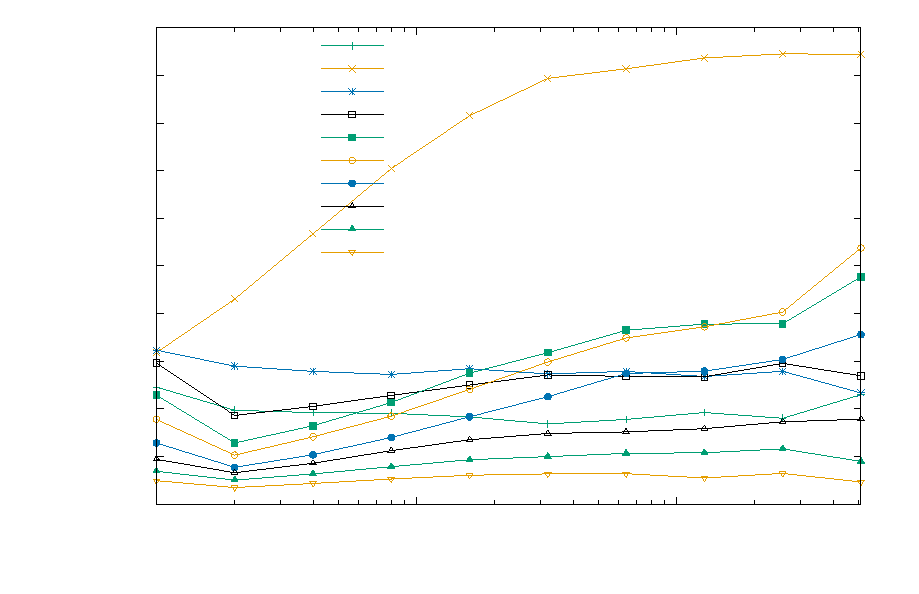
\includegraphics{bootstrap_t}}%
    \gplfronttext
  \end{picture}%
\endgroup

	\caption[error for different bin lengths]{error from the bootstrapping of binned data for several bin lengths for $N=15$}
	\label{fig:bootstrap}
\end{figure}

\begin{figure}[htbp]
	% GNUPLOT: LaTeX picture with Postscript
\begingroup
  \makeatletter
  \providecommand\color[2][]{%
    \GenericError{(gnuplot) \space\space\space\@spaces}{%
      Package color not loaded in conjunction with
      terminal option `colourtext'%
    }{See the gnuplot documentation for explanation.%
    }{Either use 'blacktext' in gnuplot or load the package
      color.sty in LaTeX.}%
    \renewcommand\color[2][]{}%
  }%
  \providecommand\includegraphics[2][]{%
    \GenericError{(gnuplot) \space\space\space\@spaces}{%
      Package graphicx or graphics not loaded%
    }{See the gnuplot documentation for explanation.%
    }{The gnuplot epslatex terminal needs graphicx.sty or graphics.sty.}%
    \renewcommand\includegraphics[2][]{}%
  }%
  \providecommand\rotatebox[2]{#2}%
  \@ifundefined{ifGPcolor}{%
    \newif\ifGPcolor
    \GPcolortrue
  }{}%
  \@ifundefined{ifGPblacktext}{%
    \newif\ifGPblacktext
    \GPblacktextfalse
  }{}%
  % define a \g@addto@macro without @ in the name:
  \let\gplgaddtomacro\g@addto@macro
  % define empty templates for all commands taking text:
  \gdef\gplbacktext{}%
  \gdef\gplfronttext{}%
  \makeatother
  \ifGPblacktext
    % no textcolor at all
    \def\colorrgb#1{}%
    \def\colorgray#1{}%
  \else
    % gray or color?
    \ifGPcolor
      \def\colorrgb#1{\color[rgb]{#1}}%
      \def\colorgray#1{\color[gray]{#1}}%
      \expandafter\def\csname LTw\endcsname{\color{white}}%
      \expandafter\def\csname LTb\endcsname{\color{black}}%
      \expandafter\def\csname LTa\endcsname{\color{black}}%
      \expandafter\def\csname LT0\endcsname{\color[rgb]{1,0,0}}%
      \expandafter\def\csname LT1\endcsname{\color[rgb]{0,1,0}}%
      \expandafter\def\csname LT2\endcsname{\color[rgb]{0,0,1}}%
      \expandafter\def\csname LT3\endcsname{\color[rgb]{1,0,1}}%
      \expandafter\def\csname LT4\endcsname{\color[rgb]{0,1,1}}%
      \expandafter\def\csname LT5\endcsname{\color[rgb]{1,1,0}}%
      \expandafter\def\csname LT6\endcsname{\color[rgb]{0,0,0}}%
      \expandafter\def\csname LT7\endcsname{\color[rgb]{1,0.3,0}}%
      \expandafter\def\csname LT8\endcsname{\color[rgb]{0.5,0.5,0.5}}%
    \else
      % gray
      \def\colorrgb#1{\color{black}}%
      \def\colorgray#1{\color[gray]{#1}}%
      \expandafter\def\csname LTw\endcsname{\color{white}}%
      \expandafter\def\csname LTb\endcsname{\color{black}}%
      \expandafter\def\csname LTa\endcsname{\color{black}}%
      \expandafter\def\csname LT0\endcsname{\color{black}}%
      \expandafter\def\csname LT1\endcsname{\color{black}}%
      \expandafter\def\csname LT2\endcsname{\color{black}}%
      \expandafter\def\csname LT3\endcsname{\color{black}}%
      \expandafter\def\csname LT4\endcsname{\color{black}}%
      \expandafter\def\csname LT5\endcsname{\color{black}}%
      \expandafter\def\csname LT6\endcsname{\color{black}}%
      \expandafter\def\csname LT7\endcsname{\color{black}}%
      \expandafter\def\csname LT8\endcsname{\color{black}}%
    \fi
  \fi
    \setlength{\unitlength}{0.0500bp}%
    \ifx\gptboxheight\undefined%
      \newlength{\gptboxheight}%
      \newlength{\gptboxwidth}%
      \newsavebox{\gptboxtext}%
    \fi%
    \setlength{\fboxrule}{0.5pt}%
    \setlength{\fboxsep}{1pt}%
\begin{picture}(8502.00,5668.00)%
    \gplgaddtomacro\gplbacktext{%
      \csname LTb\endcsname%
      \put(946,704){\makebox(0,0)[r]{\strut{}$10^{-4}$}}%
      \csname LTb\endcsname%
      \put(946,1319){\makebox(0,0)[r]{\strut{}$10^{-3}$}}%
      \csname LTb\endcsname%
      \put(946,1933){\makebox(0,0)[r]{\strut{}$10^{-2}$}}%
      \csname LTb\endcsname%
      \put(946,2548){\makebox(0,0)[r]{\strut{}$10^{-1}$}}%
      \csname LTb\endcsname%
      \put(946,3163){\makebox(0,0)[r]{\strut{}$10^{0}$}}%
      \csname LTb\endcsname%
      \put(946,3778){\makebox(0,0)[r]{\strut{}$10^{1}$}}%
      \csname LTb\endcsname%
      \put(946,4392){\makebox(0,0)[r]{\strut{}$10^{2}$}}%
      \csname LTb\endcsname%
      \put(946,5007){\makebox(0,0)[r]{\strut{}$10^{3}$}}%
      \csname LTb\endcsname%
      \put(1078,484){\makebox(0,0){\strut{}$0$}}%
      \csname LTb\endcsname%
      \put(1781,484){\makebox(0,0){\strut{}$10$}}%
      \csname LTb\endcsname%
      \put(2483,484){\makebox(0,0){\strut{}$20$}}%
      \csname LTb\endcsname%
      \put(3186,484){\makebox(0,0){\strut{}$30$}}%
      \csname LTb\endcsname%
      \put(3889,484){\makebox(0,0){\strut{}$40$}}%
      \csname LTb\endcsname%
      \put(4592,484){\makebox(0,0){\strut{}$50$}}%
      \csname LTb\endcsname%
      \put(5294,484){\makebox(0,0){\strut{}$60$}}%
      \csname LTb\endcsname%
      \put(5997,484){\makebox(0,0){\strut{}$70$}}%
      \csname LTb\endcsname%
      \put(6700,484){\makebox(0,0){\strut{}$80$}}%
      \csname LTb\endcsname%
      \put(7402,484){\makebox(0,0){\strut{}$90$}}%
      \csname LTb\endcsname%
      \put(8105,484){\makebox(0,0){\strut{}$100$}}%
    }%
    \gplgaddtomacro\gplfronttext{%
      \csname LTb\endcsname%
      \put(176,2855){\rotatebox{-270}{\makebox(0,0){\strut{}$|\frac{H[p_f,\phi_f]-H[p_0,\phi_0]}{H[p_0,\phi_0]}|$}}}%
      \put(4591,154){\makebox(0,0){\strut{}$N_{md}$}}%
      \put(4591,5337){\makebox(0,0){\strut{}Convergence check}}%
      \csname LTb\endcsname%
      \put(3058,4834){\makebox(0,0)[r]{\strut{}Leapfrog error}}%
    }%
    \gplbacktext
    \put(0,0){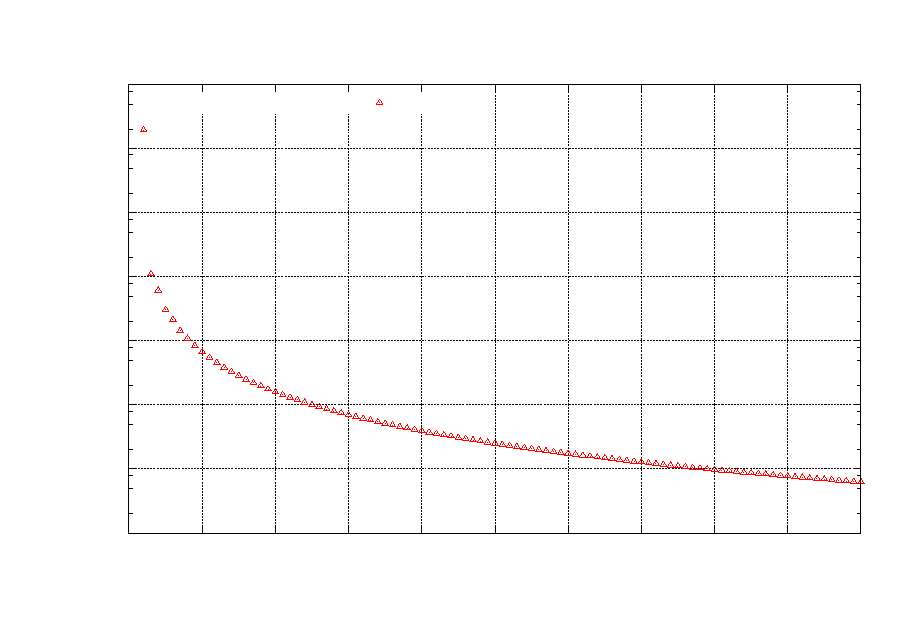
\includegraphics{converge_t}}%
    \gplfronttext
  \end{picture}%
\endgroup

	\caption{convergence of the leapfrog algorithm}
	\label{fig:converge}
\end{figure}

\section{Results}

\subsection{Convergence of leapfrog}

The convergence of our leapfrog algorithm is shown in fig.~\ref{fig:converge}. Qualitatively, it behaves the same as the expected one on the sheet: We start with a high value of $\Delta$, and it gets smaller with each step we add to the algorithm. 

Depending on our starting parameters, $\Delta$ is shifted by about one order of magnitude, which also explains why our values are different from the ones on the sheet.
We see that our leapfrog algorithm converges quite nicely and so we can use it for the rest of our calculations.


Our acceptance rates are quite high for large $N_{md}$, so we choose $N_{md}=4$ to get an acceptance rate of about 90\%. This is a bit higher than the range of acceptance rates we aim for, but the results do not follow our expectations as good for smaller $N_{md}$.
%plot description tuning of acceptance rate
\subsection{Magnetization}

The analytical expectation and our measurements for the magnetization are plotted in fig.~\ref{fig:magnetization}. We expect the magnetization to be about $0.5$ for $J=0.2$, and then rise monotonously. This rise gets less steep for growing $J$, and does not reach $m=1$. For smaller $N$, we expect the magnetization to be smaller and its rise to be less steep than for larger $N$, however the distance between the lines decreases for growing $N$.

Almost all of our measurements lie on the expected curves, there are some outliers for small $J$ or small $N$. The erorrs are quite small for all $J$, and a bit bigger when the measurements are further away from the curve.

The errors are quite small for all $N$, but they rise for smaller $N$.
\begin{figure}[htbp]
	% GNUPLOT: LaTeX picture with Postscript
\begingroup
  \makeatletter
  \providecommand\color[2][]{%
    \GenericError{(gnuplot) \space\space\space\@spaces}{%
      Package color not loaded in conjunction with
      terminal option `colourtext'%
    }{See the gnuplot documentation for explanation.%
    }{Either use 'blacktext' in gnuplot or load the package
      color.sty in LaTeX.}%
    \renewcommand\color[2][]{}%
  }%
  \providecommand\includegraphics[2][]{%
    \GenericError{(gnuplot) \space\space\space\@spaces}{%
      Package graphicx or graphics not loaded%
    }{See the gnuplot documentation for explanation.%
    }{The gnuplot epslatex terminal needs graphicx.sty or graphics.sty.}%
    \renewcommand\includegraphics[2][]{}%
  }%
  \providecommand\rotatebox[2]{#2}%
  \@ifundefined{ifGPcolor}{%
    \newif\ifGPcolor
    \GPcolortrue
  }{}%
  \@ifundefined{ifGPblacktext}{%
    \newif\ifGPblacktext
    \GPblacktextfalse
  }{}%
  % define a \g@addto@macro without @ in the name:
  \let\gplgaddtomacro\g@addto@macro
  % define empty templates for all commands taking text:
  \gdef\gplbacktext{}%
  \gdef\gplfronttext{}%
  \makeatother
  \ifGPblacktext
    % no textcolor at all
    \def\colorrgb#1{}%
    \def\colorgray#1{}%
  \else
    % gray or color?
    \ifGPcolor
      \def\colorrgb#1{\color[rgb]{#1}}%
      \def\colorgray#1{\color[gray]{#1}}%
      \expandafter\def\csname LTw\endcsname{\color{white}}%
      \expandafter\def\csname LTb\endcsname{\color{black}}%
      \expandafter\def\csname LTa\endcsname{\color{black}}%
      \expandafter\def\csname LT0\endcsname{\color[rgb]{1,0,0}}%
      \expandafter\def\csname LT1\endcsname{\color[rgb]{0,1,0}}%
      \expandafter\def\csname LT2\endcsname{\color[rgb]{0,0,1}}%
      \expandafter\def\csname LT3\endcsname{\color[rgb]{1,0,1}}%
      \expandafter\def\csname LT4\endcsname{\color[rgb]{0,1,1}}%
      \expandafter\def\csname LT5\endcsname{\color[rgb]{1,1,0}}%
      \expandafter\def\csname LT6\endcsname{\color[rgb]{0,0,0}}%
      \expandafter\def\csname LT7\endcsname{\color[rgb]{1,0.3,0}}%
      \expandafter\def\csname LT8\endcsname{\color[rgb]{0.5,0.5,0.5}}%
    \else
      % gray
      \def\colorrgb#1{\color{black}}%
      \def\colorgray#1{\color[gray]{#1}}%
      \expandafter\def\csname LTw\endcsname{\color{white}}%
      \expandafter\def\csname LTb\endcsname{\color{black}}%
      \expandafter\def\csname LTa\endcsname{\color{black}}%
      \expandafter\def\csname LT0\endcsname{\color{black}}%
      \expandafter\def\csname LT1\endcsname{\color{black}}%
      \expandafter\def\csname LT2\endcsname{\color{black}}%
      \expandafter\def\csname LT3\endcsname{\color{black}}%
      \expandafter\def\csname LT4\endcsname{\color{black}}%
      \expandafter\def\csname LT5\endcsname{\color{black}}%
      \expandafter\def\csname LT6\endcsname{\color{black}}%
      \expandafter\def\csname LT7\endcsname{\color{black}}%
      \expandafter\def\csname LT8\endcsname{\color{black}}%
    \fi
  \fi
    \setlength{\unitlength}{0.0500bp}%
    \ifx\gptboxheight\undefined%
      \newlength{\gptboxheight}%
      \newlength{\gptboxwidth}%
      \newsavebox{\gptboxtext}%
    \fi%
    \setlength{\fboxrule}{0.5pt}%
    \setlength{\fboxsep}{1pt}%
\begin{picture}(8502.00,5668.00)%
    \gplgaddtomacro\gplbacktext{%
      \csname LTb\endcsname%
      \put(814,704){\makebox(0,0)[r]{\strut{}$0$}}%
      \csname LTb\endcsname%
      \put(814,1644){\makebox(0,0)[r]{\strut{}$0.2$}}%
      \csname LTb\endcsname%
      \put(814,2584){\makebox(0,0)[r]{\strut{}$0.4$}}%
      \csname LTb\endcsname%
      \put(814,3523){\makebox(0,0)[r]{\strut{}$0.6$}}%
      \csname LTb\endcsname%
      \put(814,4463){\makebox(0,0)[r]{\strut{}$0.8$}}%
      \csname LTb\endcsname%
      \put(814,5403){\makebox(0,0)[r]{\strut{}$1$}}%
      \csname LTb\endcsname%
      \put(946,484){\makebox(0,0){\strut{}$0.2$}}%
      \csname LTb\endcsname%
      \put(1741,484){\makebox(0,0){\strut{}$0.4$}}%
      \csname LTb\endcsname%
      \put(2537,484){\makebox(0,0){\strut{}$0.6$}}%
      \csname LTb\endcsname%
      \put(3332,484){\makebox(0,0){\strut{}$0.8$}}%
      \csname LTb\endcsname%
      \put(4128,484){\makebox(0,0){\strut{}$1$}}%
      \csname LTb\endcsname%
      \put(4923,484){\makebox(0,0){\strut{}$1.2$}}%
      \csname LTb\endcsname%
      \put(5719,484){\makebox(0,0){\strut{}$1.4$}}%
      \csname LTb\endcsname%
      \put(6514,484){\makebox(0,0){\strut{}$1.6$}}%
      \csname LTb\endcsname%
      \put(7310,484){\makebox(0,0){\strut{}$1.8$}}%
      \csname LTb\endcsname%
      \put(8105,484){\makebox(0,0){\strut{}$2$}}%
    }%
    \gplgaddtomacro\gplfronttext{%
      \csname LTb\endcsname%
      \put(176,3053){\rotatebox{-270}{\makebox(0,0){\strut{}$\langle m \rangle$}}}%
      \put(4525,154){\makebox(0,0){\strut{}$J$}}%
      \put(4525,5293){\makebox(0,0){\strut{}}}%
      \csname LTb\endcsname%
      \put(7118,1537){\makebox(0,0)[r]{\strut{}$N=$5}}%
      \csname LTb\endcsname%
      \put(7118,1317){\makebox(0,0)[r]{\strut{}$N=$10}}%
      \csname LTb\endcsname%
      \put(7118,1097){\makebox(0,0)[r]{\strut{}$N=$15}}%
      \csname LTb\endcsname%
      \put(7118,877){\makebox(0,0)[r]{\strut{}$N=$20}}%
    }%
    \gplbacktext
    \put(0,0){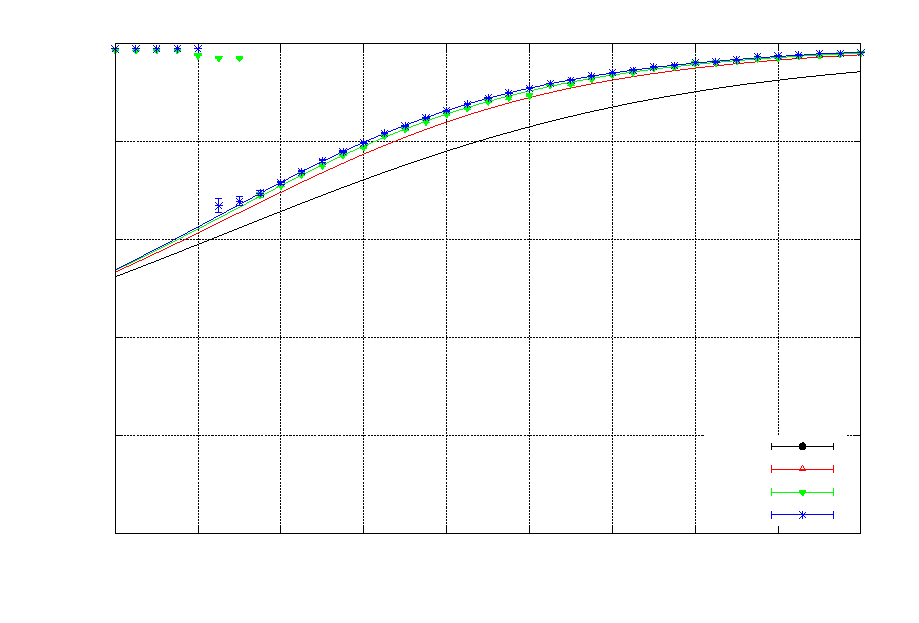
\includegraphics{magnetization_t}}%
    \gplfronttext
  \end{picture}%
\endgroup

	\caption{magnetization for different $N$}
	\label{fig:magnetization}
\end{figure}
%plot description

\subsection{Average energy per site}

The expected values and our measurements for $\langle \beta\epsilon\rangle$ are plotted in fig.~\ref{fig:energy}. We expect $\langle \beta\epsilon\rangle\approx-0.3$ for $J=0.2$, and for the energy to decrease monotonously, with almost a constant descent. We also expect the energy levels of the different $N$ to grow further apart for growing $J$, and for the energy to be higher for smaller $N$.

Again, our measurements are close to the expectations, most points lie on the expected curve. There are some outliers for small $J$ and the ponts with $N=5$ seem to \enquote{wobble} around the expected curve a bit, but still have the same behavior.
The errors are quite small, even for those points which do not lie on the curve.
  
\begin{figure}[htbp]
	% GNUPLOT: LaTeX picture with Postscript
\begingroup
  \makeatletter
  \providecommand\color[2][]{%
    \GenericError{(gnuplot) \space\space\space\@spaces}{%
      Package color not loaded in conjunction with
      terminal option `colourtext'%
    }{See the gnuplot documentation for explanation.%
    }{Either use 'blacktext' in gnuplot or load the package
      color.sty in LaTeX.}%
    \renewcommand\color[2][]{}%
  }%
  \providecommand\includegraphics[2][]{%
    \GenericError{(gnuplot) \space\space\space\@spaces}{%
      Package graphicx or graphics not loaded%
    }{See the gnuplot documentation for explanation.%
    }{The gnuplot epslatex terminal needs graphicx.sty or graphics.sty.}%
    \renewcommand\includegraphics[2][]{}%
  }%
  \providecommand\rotatebox[2]{#2}%
  \@ifundefined{ifGPcolor}{%
    \newif\ifGPcolor
    \GPcolortrue
  }{}%
  \@ifundefined{ifGPblacktext}{%
    \newif\ifGPblacktext
    \GPblacktextfalse
  }{}%
  % define a \g@addto@macro without @ in the name:
  \let\gplgaddtomacro\g@addto@macro
  % define empty templates for all commands taking text:
  \gdef\gplbacktext{}%
  \gdef\gplfronttext{}%
  \makeatother
  \ifGPblacktext
    % no textcolor at all
    \def\colorrgb#1{}%
    \def\colorgray#1{}%
  \else
    % gray or color?
    \ifGPcolor
      \def\colorrgb#1{\color[rgb]{#1}}%
      \def\colorgray#1{\color[gray]{#1}}%
      \expandafter\def\csname LTw\endcsname{\color{white}}%
      \expandafter\def\csname LTb\endcsname{\color{black}}%
      \expandafter\def\csname LTa\endcsname{\color{black}}%
      \expandafter\def\csname LT0\endcsname{\color[rgb]{1,0,0}}%
      \expandafter\def\csname LT1\endcsname{\color[rgb]{0,1,0}}%
      \expandafter\def\csname LT2\endcsname{\color[rgb]{0,0,1}}%
      \expandafter\def\csname LT3\endcsname{\color[rgb]{1,0,1}}%
      \expandafter\def\csname LT4\endcsname{\color[rgb]{0,1,1}}%
      \expandafter\def\csname LT5\endcsname{\color[rgb]{1,1,0}}%
      \expandafter\def\csname LT6\endcsname{\color[rgb]{0,0,0}}%
      \expandafter\def\csname LT7\endcsname{\color[rgb]{1,0.3,0}}%
      \expandafter\def\csname LT8\endcsname{\color[rgb]{0.5,0.5,0.5}}%
    \else
      % gray
      \def\colorrgb#1{\color{black}}%
      \def\colorgray#1{\color[gray]{#1}}%
      \expandafter\def\csname LTw\endcsname{\color{white}}%
      \expandafter\def\csname LTb\endcsname{\color{black}}%
      \expandafter\def\csname LTa\endcsname{\color{black}}%
      \expandafter\def\csname LT0\endcsname{\color{black}}%
      \expandafter\def\csname LT1\endcsname{\color{black}}%
      \expandafter\def\csname LT2\endcsname{\color{black}}%
      \expandafter\def\csname LT3\endcsname{\color{black}}%
      \expandafter\def\csname LT4\endcsname{\color{black}}%
      \expandafter\def\csname LT5\endcsname{\color{black}}%
      \expandafter\def\csname LT6\endcsname{\color{black}}%
      \expandafter\def\csname LT7\endcsname{\color{black}}%
      \expandafter\def\csname LT8\endcsname{\color{black}}%
    \fi
  \fi
    \setlength{\unitlength}{0.0500bp}%
    \ifx\gptboxheight\undefined%
      \newlength{\gptboxheight}%
      \newlength{\gptboxwidth}%
      \newsavebox{\gptboxtext}%
    \fi%
    \setlength{\fboxrule}{0.5pt}%
    \setlength{\fboxsep}{1pt}%
\begin{picture}(8502.00,5668.00)%
    \gplgaddtomacro\gplbacktext{%
      \csname LTb\endcsname%%
      \put(814,704){\makebox(0,0)[r]{\strut{}$-14$}}%
      \csname LTb\endcsname%%
      \put(814,1382){\makebox(0,0)[r]{\strut{}$-12$}}%
      \csname LTb\endcsname%%
      \put(814,2059){\makebox(0,0)[r]{\strut{}$-10$}}%
      \csname LTb\endcsname%%
      \put(814,2737){\makebox(0,0)[r]{\strut{}$-8$}}%
      \csname LTb\endcsname%%
      \put(814,3414){\makebox(0,0)[r]{\strut{}$-6$}}%
      \csname LTb\endcsname%%
      \put(814,4092){\makebox(0,0)[r]{\strut{}$-4$}}%
      \csname LTb\endcsname%%
      \put(814,4769){\makebox(0,0)[r]{\strut{}$-2$}}%
      \csname LTb\endcsname%%
      \put(814,5447){\makebox(0,0)[r]{\strut{}$0$}}%
      \csname LTb\endcsname%%
      \put(946,484){\makebox(0,0){\strut{}$0.2$}}%
      \csname LTb\endcsname%%
      \put(1741,484){\makebox(0,0){\strut{}$0.4$}}%
      \csname LTb\endcsname%%
      \put(2537,484){\makebox(0,0){\strut{}$0.6$}}%
      \csname LTb\endcsname%%
      \put(3332,484){\makebox(0,0){\strut{}$0.8$}}%
      \csname LTb\endcsname%%
      \put(4128,484){\makebox(0,0){\strut{}$1$}}%
      \csname LTb\endcsname%%
      \put(4923,484){\makebox(0,0){\strut{}$1.2$}}%
      \csname LTb\endcsname%%
      \put(5719,484){\makebox(0,0){\strut{}$1.4$}}%
      \csname LTb\endcsname%%
      \put(6514,484){\makebox(0,0){\strut{}$1.6$}}%
      \csname LTb\endcsname%%
      \put(7310,484){\makebox(0,0){\strut{}$1.8$}}%
      \csname LTb\endcsname%%
      \put(8105,484){\makebox(0,0){\strut{}$2$}}%
    }%
    \gplgaddtomacro\gplfronttext{%
      \csname LTb\endcsname%%
      \put(198,3075){\rotatebox{-270}{\makebox(0,0){\strut{}$\langle \beta\epsilon \rangle$}}}%
      \put(4525,154){\makebox(0,0){\strut{}$J$}}%
      \put(4525,5337){\makebox(0,0){\strut{}}}%
      \csname LTb\endcsname%%
      \put(7118,5274){\makebox(0,0)[r]{\strut{}$N=$5}}%
      \csname LTb\endcsname%%
      \put(7118,5054){\makebox(0,0)[r]{\strut{}$N=$10}}%
      \csname LTb\endcsname%%
      \put(7118,4834){\makebox(0,0)[r]{\strut{}$N=$15}}%
      \csname LTb\endcsname%%
      \put(7118,4614){\makebox(0,0)[r]{\strut{}$N=$20}}%
    }%
    \gplbacktext
    \put(0,0){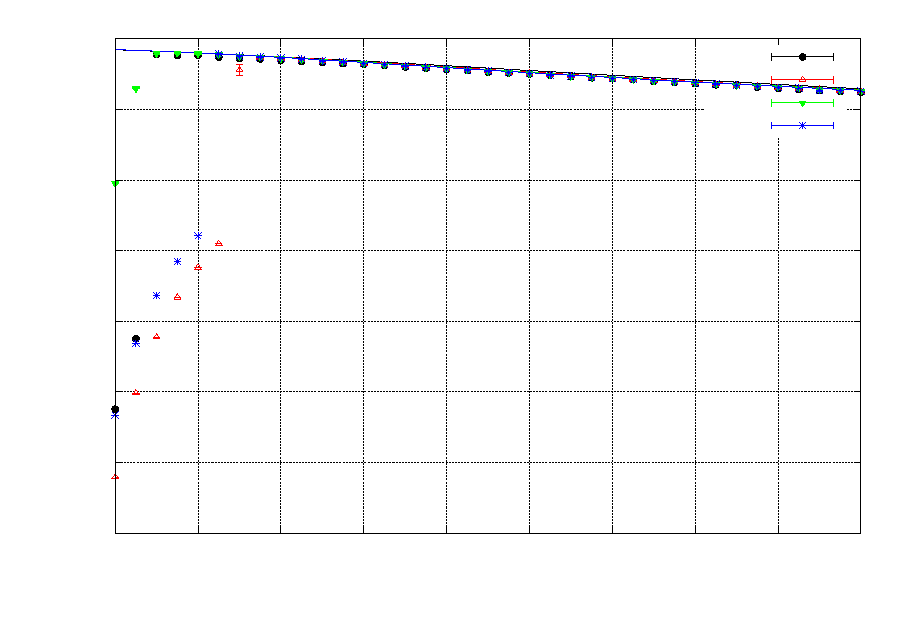
\includegraphics{energy_t}}%
    \gplfronttext
  \end{picture}%
\endgroup

	\caption{energy per site for different $N$}
	\label{fig:energy}
\end{figure}
%plot description

The results for the average energy per site are not as close to the expectation as those for the magnetization, however both reproduce the analytical results, and thus show that the HMC-algorithm coupled with leapfrog can be quite a powerful tool.

\newpage	
\listoffigures
\printbibliography
\end{document}